%! Author = Len Washington III
%! Date = 1/28/24

% Preamble
\documentclass[title={Chapter 3}]{fdsn201notes}

% Packages

% Document
\begin{document}

\maketitle{3}

\section{Organization of the Body}\label{sec:organization-of-the-body}
\definition{Atoms}{the smallest units of matter}
\begin{itemize}
	\item Atoms bond to each other to form molecules
\end{itemize}
\definition{Molecules}{groups of atoms bonded in specific configurations}
\begin{itemize}
	\item Examples
	\begin{itemize}
		\item Water is $\mbox{H}_{2}\mbox{O}$
		\item Carbon dioxide is $\mbox{CO}_{2}$
	\end{itemize}
	\item Carbohydrates, proteins, fats, and vitamins are usually very large molecules
	\item The goal of digestion:
	\begin{itemize}
		\item Break these large molecules down into smaller molecules
		\item Absorb the smaller molecules into the cells of the body
	\end{itemize}
\end{itemize}

\begin{figure}[H]
	\centering
	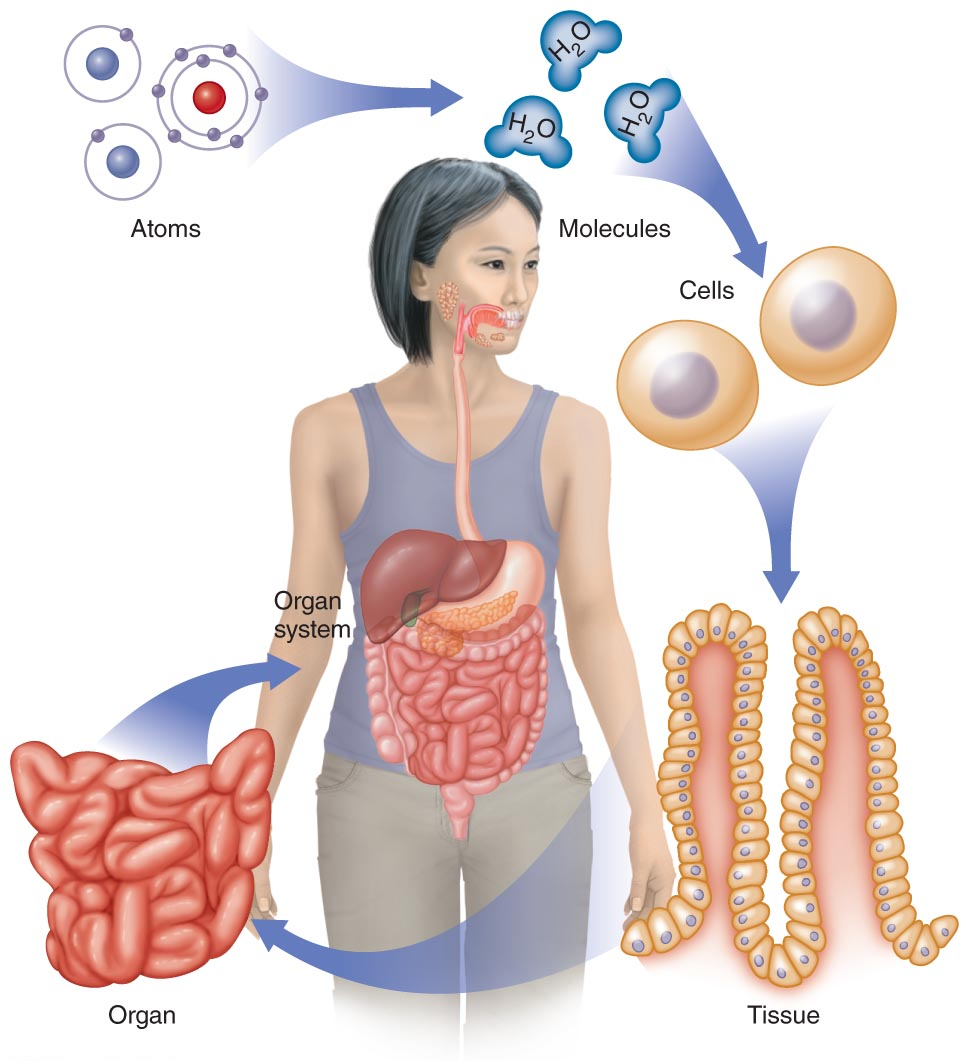
\includegraphics[width=\textwidth]{3_digestion}
	\caption{}
	\label{fig:3_digestion}
\end{figure}

\begin{itemize}
	\item Molecules are the building blocks of cells
	\item \definition{Cells}{the smallest unit of life}
	\item Molecules that result from the digestion of food are used to build the cells of the body
	\item \definition{Cell membrane}{outer layer enclosing each cell of the body}
	\begin{itemize}
		\item Composed of two layers of phospholipids
		\item Long lipid ``tails'' face each other toward the interior of the membrane
		\item Phosphate ``heads'' line the interior and exterior surfaces of the membrane
		\item Cholesterol and proteins are embedded in the membrane
	\end{itemize}
	\item The cell membrane is \textcolor{red}{selectively permeable}, allowing it to control the passage of materials into and out of the cell
	\item The cell membrane encloses the
	\begin{itemize}
		\item \definition{Cytoplasm}{the liquid within the cell}
		\item \definition{Organelles}{tiny structures that perform many different cellular functions}
		\item Examples
		\begin{itemize}
			\item Nucleus
			\item Mitochondria
		\end{itemize}
	\end{itemize}
\end{itemize}

\begin{figure}[H]
	\centering
	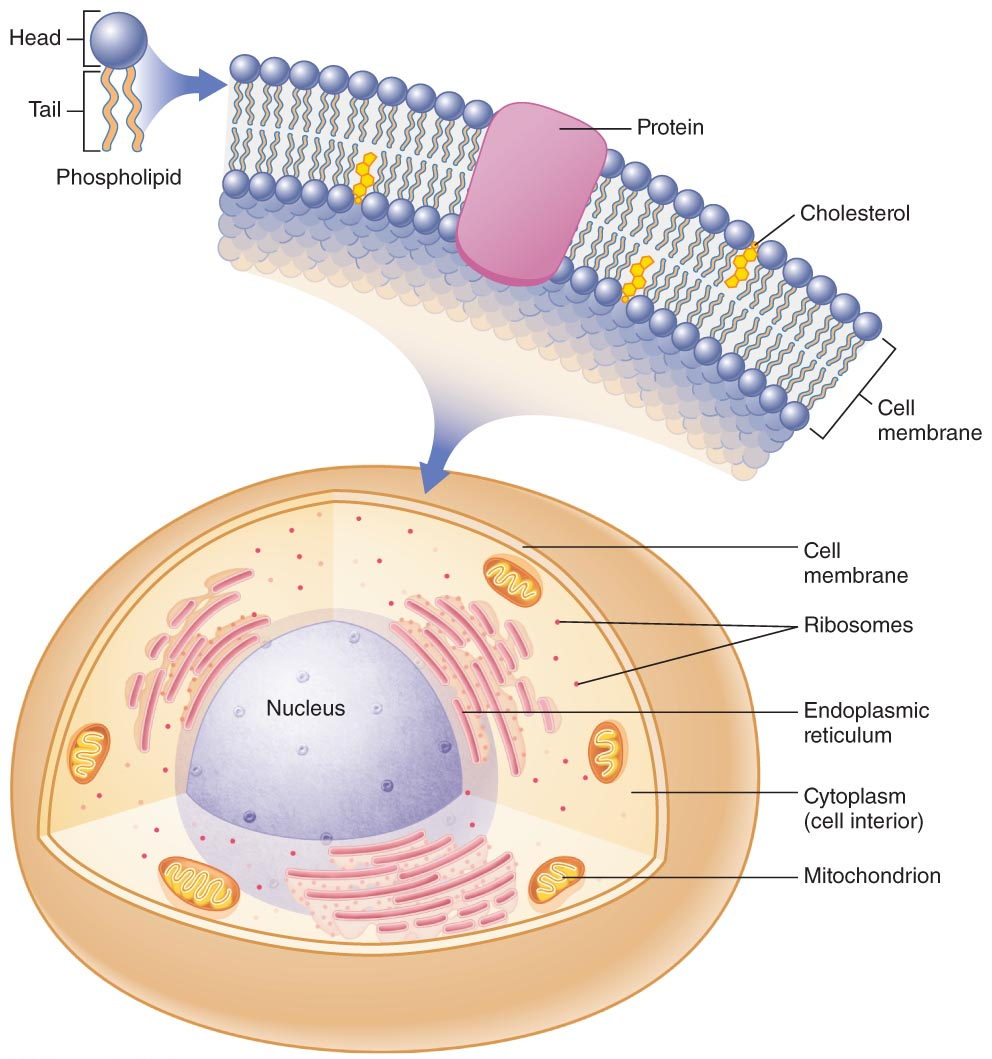
\includegraphics[width=\textwidth]{3_representative_enterocyte}
	\caption{Representative Enterocyte}
	\label{fig:representative-enterocyte}
\end{figure}

\begin{itemize}
	\item Cells join together to form tissues
	\item \definition{Tissue}{group of cells acting together to perform a common function}
	\begin{itemize}
		\item Examples
		\begin{itemize}
			\item Muscle tissue
			\item Nervous tissue
		\end{itemize}
	\end{itemize}
\end{itemize}

\begin{itemize}
	\item Different tissues combine to form organs
	\item \definition{Organ}{a sophisticated organization of tissues that performs a specific function}
	\begin{itemize}
		\item Examples
		\begin{itemize}
			\item Stomach
			\item Heart
			\item Brain
		\end{itemize}
	\end{itemize}
	\item \definition{Organ systems}{groups of organs working together for a particular function}
	\begin{itemize}
		\item Example
		\begin{itemize}
			\item Gastrointestinal system
		\end{itemize}
	\end{itemize}
\end{itemize}

\section{Types of Organ Systems (11)}\label{sec:types-of-organ-systems-(11)}
\begin{itemize}
	\item Nervous
	\item Cardiovascular (circulatory)
	\item Respiratory
	\item Renal
	\item Digestive
	\item Endocrine
	\item Integumentary \& Exocrine
	\item Immune \& Lymphatic
	\item Muscular
	\item Skeletal
	\item Reproductive
\end{itemize}

\section{Why Do We Want to Eat?}\label{sec:why-do-we-want-to-eat?}
\definition{Appetite}{a desire to eat that is stimulated by}
\begin{itemize}
	\item Sight
	\item Smell
	\item Thought of food
\end{itemize}
\definition{Hunger}{a physiologic drive to eat that occurs when our body senses that we need food}
\begin{itemize}
	\item The \textcolor{red}{hypothalamus} region of the brain contains a cluster of nerve cells known as the feeding center and another cluster of cells known as the satiety center
	\begin{itemize}
		\item Nerve cells in the stomach and small intestine sense food and send message to hypothalamus
		\item Hormones relay messages to the hypothalamus
		\item Amount and type of food consumed influence satiety
	\end{itemize}
\end{itemize}

\begin{figure}[H]
	\centering
	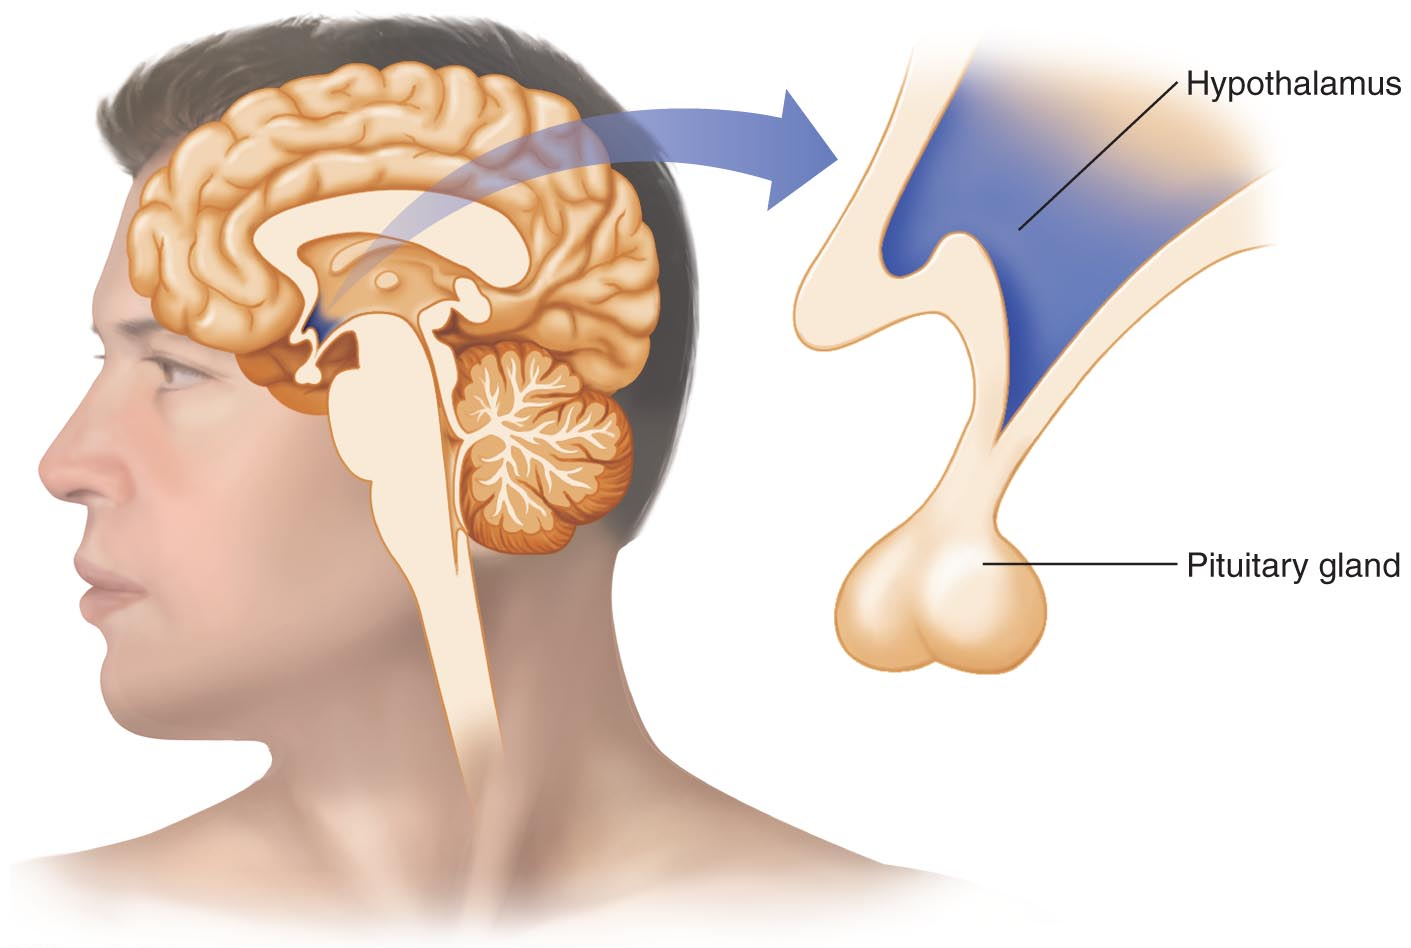
\includegraphics[width=\textwidth]{3_hypothalamus}
	\caption{The Hypothalamus Triggers Hunger}
	\label{fig:hypothalamus-triggers-hunger}
\end{figure}

\begin{itemize}
	\item The signals that prompt us to eat include
	\begin{itemize}
		\item Nerve receptors in the stomach, which send signals to the hypothalamus to indicate if the stomach is full ot empty
		\item Blood fuel (glucose, ketones) levels, which trigger the release of hormones
		\begin{itemize}
			\item insulin and glucagon
		\end{itemize}
	\end{itemize}
	\item \definition{Hormones}{chemicals produced in specialized glands that travel in the bloodstream to target organs in other parts of the body}
	\begin{itemize}
		\item Some hormones stimulate hunger
		\begin{itemize}
			\item Ghrelin
		\end{itemize}
		\item Some hormones produce a feeling of satiety
		\begin{itemize}
			\item Cholecystokinin (CCK)
			\item Leptin
		\end{itemize}
	\end{itemize}
	\item Foods have different effects on our feelings of hunger and satiety
	\begin{itemize}
		\item Proteins have the highest satiety value
		\item Carbohydrates have a lower satiety value than fats
		\item Bulky foods provided a sense of satiety
		\item Solid foods are more filling than semisolid foods or liquids
	\end{itemize}
\end{itemize}

\section{What Happens to the Food We Eat?}\label{sec:what-happens-to-the-food-we-eat?}
\begin{itemize}
	\item \definition{Gastrointestinal (GI) tract}{series of organs arranged as a long tube through which the food passes}
	\item The GI tract includes
	\begin{itemize}
		\item Organs such as the stomach and intestines
		\item \definition{Sphincters}{muscles that control the passage of material from one organ to the next}
	\end{itemize}
\end{itemize}

\begin{figure}[H]
	\centering
	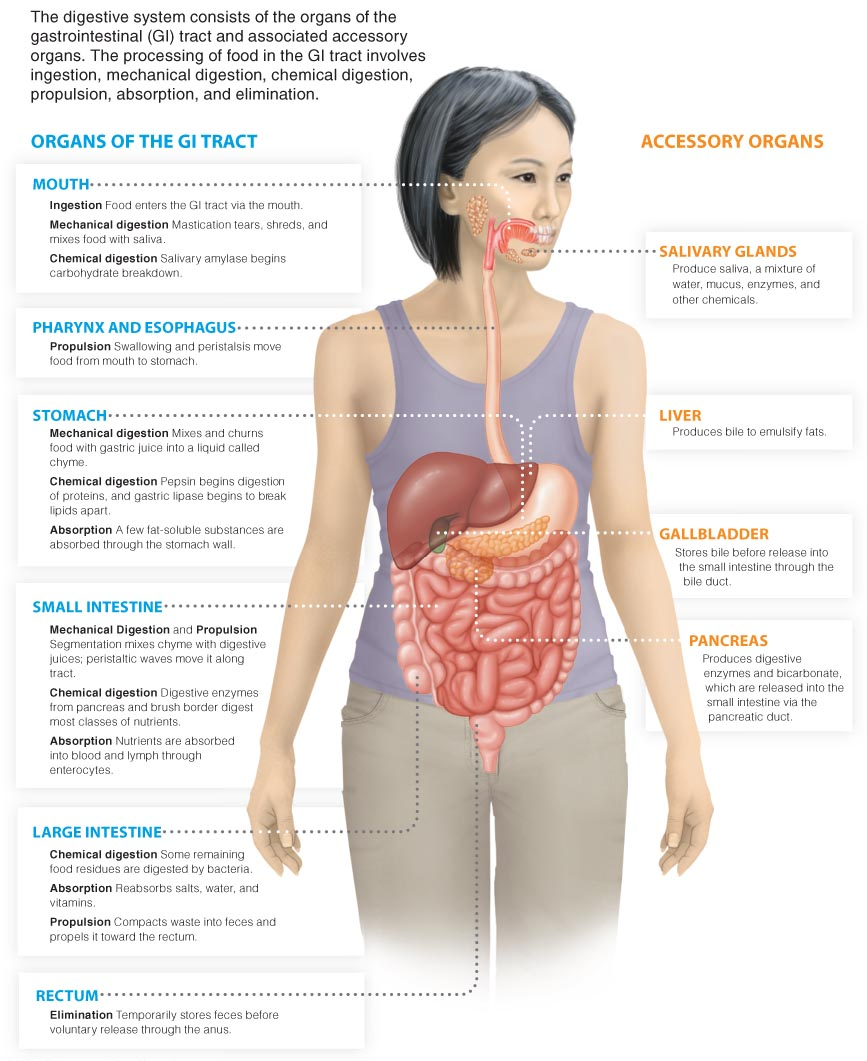
\includegraphics[width=\textwidth]{3_digestive_system}
	\caption{Digestive System}
	\label{fig:digestive-system}
\end{figure}

\section{Digestion}\label{sec:digestion}
\subsection{The Mouth}\label{subsec:digestion-the-mouth}
\begin{itemize}
	\item Digestion begins in the mouth
	\begin{itemize}
		\item Chewing is the mechanical digestion that breaks food into smaller pieces
		\item Some chemical digestion takes place in the mouth
		\begin{itemize}
			\item \definition{Salivary amylase}{an \textcolor{red}{enzyme} produced by the \textcolor{red}{salivary glands} that begins the chemical digestion of carbohydrates}
		\end{itemize}
	\end{itemize}
\end{itemize}

\begin{figure}[H]
	\centering
	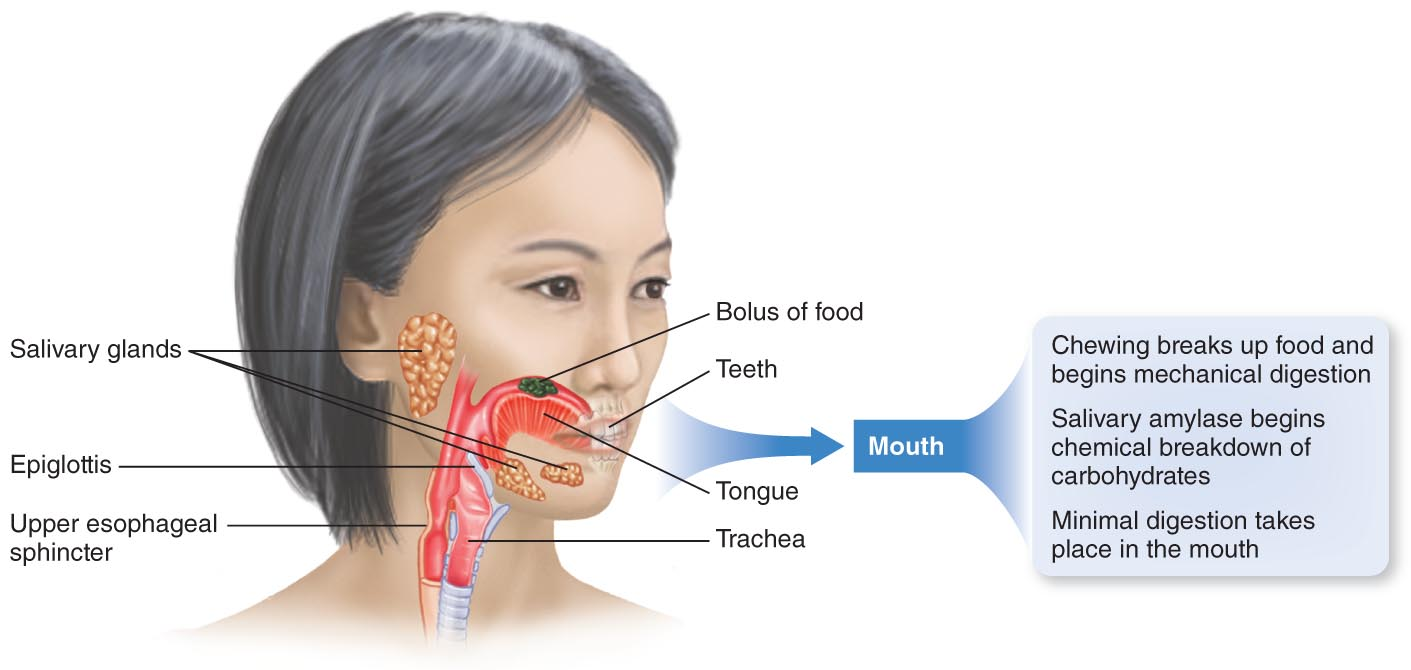
\includegraphics[width=\textwidth]{3_digestion_mouth}
	\caption{}
	\label{fig:digestion-mouth}
\end{figure}

\begin{itemize}
	\item The esophagus propels food into the stomach
	\begin{itemize}
		\item The \textcolor{red}{epiglottis} covers the opening to the trachea during swallowing
		\item Food travels from the mouth to the stomach through the \textcolor{red}{esophagus}
		\item \textcolor{red}{Peristalsis} is the muscular contractions moving food through the GI tract
		\item The \textcolor{red}{gastroesophogeal sphincter} separates the esophagus from the stomach
	\end{itemize}
\end{itemize}

\subsection{Stomach}\label{subsec:digestion-stomach}
\begin{itemize}
	\item The stomach mixes, digests, and stores food
	\item Digestion in the stomach includes
	\begin{itemize}
		\item Extensive mechanical digestion to mix food with gastric juice
		\item Chemical digestion of proteins and fats
	\end{itemize}
	\item \textcolor{red}{Gastric juice} contains
	\begin{itemize}
		\item \definition{Hydrochloric acid (HCl)}{to denature proteins and activate pepsin}
		\item \definition{Intrinsic factor}{a protein critical to the absorption of vitamin $\mbox{B}_{12}$}
		\item \definition{Pepsin}{an enzyme to digest protein}
		\item \definition{Gastric lipase}{an enzyme to digest fat}
	\end{itemize}
	\item \definition{Chyme}{semisolid product of mechanical and chemical digestion in the stomach}
\end{itemize}

\begin{figure}[H]
	\centering
	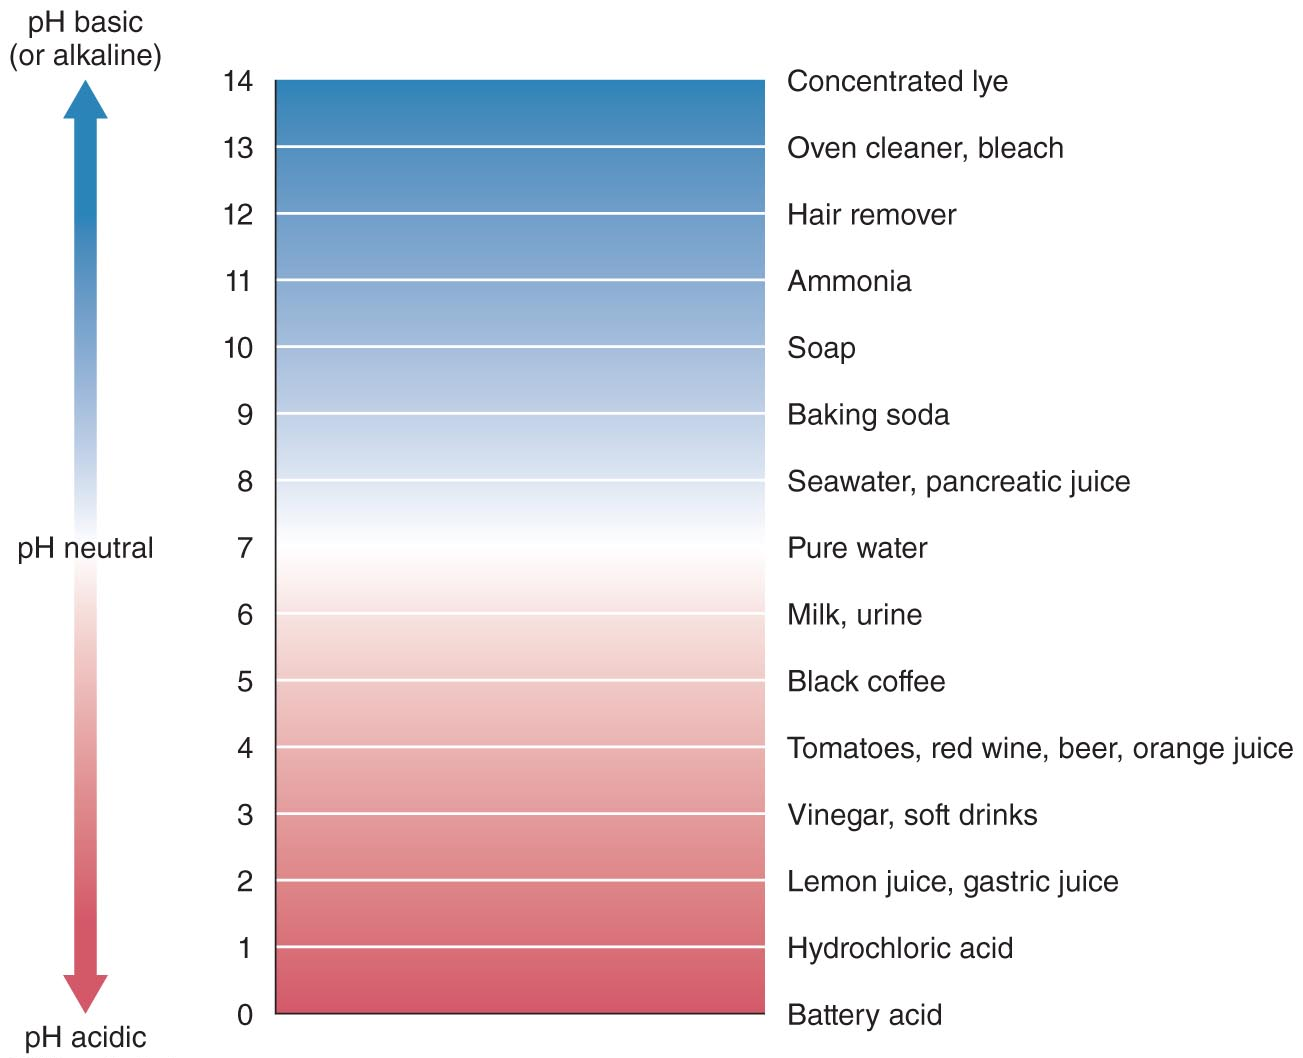
\includegraphics[width=\textwidth]{3_ph}
	\caption{Hydrochloric Acid (HCl) on the pH Scale}
	\label{fig:ph}
\end{figure}

\subsection{Small Intestine}\label{subsec:small-intestine}
\begin{itemize}
	\item From the stomach, chyme is slowly released through the pyloric sphincter to the small intestine
	\item Chemical digestion continues in the small intestine using pancreatic enzymes and bile
\end{itemize}

\subsection{Large Intestine}\label{subsec:large-intestine}
\begin{itemize}
	\item Undigested food components move through a sphincter called the \textcolor{red}{ileocecal valve} to the large intestine
	\item In the large intestine
	\begin{itemize}
		\item Very little digestion takes place
		\item Material is stored 12--24 hours prior to elimination
		\item Water and some nutrients are absorbed
	\end{itemize}
\end{itemize}

\begin{figure}[H]
	\centering
	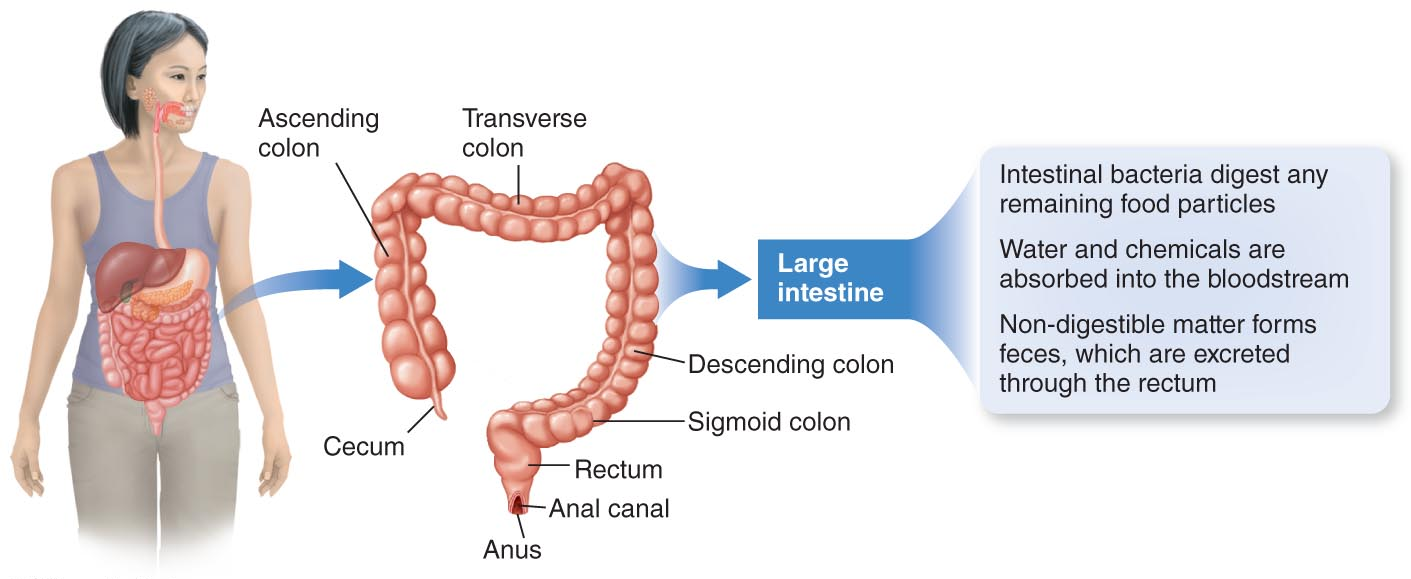
\includegraphics[width=\textwidth]{3_elimination}
	\caption{Elimination}
	\label{fig:elimination}
\end{figure}

\subsection{Accessory Organs}\label{subsec:accessory-organs}
\begin{itemize}
	\item Surrounding the GI tract are several \textcolor{red}{accessory organs}
	\begin{itemize}
		\item Salivary glands
		\item \definition{Liver}{produces bile, which emulsifies fats}
		\item \textcolor{red}{Pancreas}
		\begin{itemize}
			\item Produces many digestive enzymes
			\item Produces bicarbonate to neutralize chyme
		\end{itemize}
		\item \definition{Gallbladder}{stores bile}
	\end{itemize}
\end{itemize}

\section{Absorption}\label{sec:absorption}
\begin{itemize}
	\item \definition{Absorption}{the process of taking molecules across a cell membrane and into cells of the body}
	\item A small amount of absorption occurs in the stomach
	\item Most absorption of nutrients occurs in the three sections of the small intestine
	\begin{itemize}
		\item Duodenum
		\item Jejunum
		\item Ileum
	\end{itemize}
	\item The lining of the GI tract has special structures to facilitate absorption
	\begin{itemize}
		\item \definition{Villi}{folds in the lining that are in close contact with nutrient molecules}
		\item \definition{Brush border}{composed of microvilli that greatly increase the surface area}
	\end{itemize}
\end{itemize}

\begin{itemize}
	\item Water-soluble nutrients (carbohydrates, protein, minerals, and some vitamins) enter the \textcolor{red}{portal vein}
	\begin{itemize}
		\item The portal vein transports these nutrients to the liver
	\end{itemize}
	\item Fat-soluble nutrients (lipids and some vitamins) enter the lymphatic vessels
	\begin{itemize}
		\item Lymphatic vessels transport these nutrients directly to the bloodstream
	\end{itemize}
\end{itemize}

\begin{itemize}
	\item Nutrients are absorbed across the mucosal membrane and into the blood stream or lymph by:
	\begin{itemize}
		\item Passive diffusion
		\item Facilitated diffusion
		\item Active transport
		\item Endocytosis
	\end{itemize}
\end{itemize}

\section{The Role of the Neuromuscular System}\label{sec:the-role-of-the-neuromuscular-system}
\begin{itemize}
	\item Two components of the neuromuscular system regulate the activities of the GI tract
	\begin{itemize}
		\item The muscles of the GI tract mix and move food
		\begin{itemize}
			\item Both voluntary and involuntary muscles
		\end{itemize}
		\item Nerves control the contractions and secretions of the GI tract
		\begin{itemize}
			\item The \textcolor{red}{enteric nervous system (ENS)}
			\item Other branches of the autonomic nervous system
			\item The central nervous system (CNS)
		\end{itemize}
	\end{itemize}
\end{itemize}

\section{GI Tract Disorders}\label{sec:gi-tract-disorders}
\begin{itemize}
	\item The lining of the stomach is designed to cope with hydrochloric acid, but other regions of the GI tract are not
	\item \definition{Heartburn}{caused by hydrochloric acid in the esophagus}
	\item \definition{Gastroesophageal reflux disease (GERD)}{a chronic disease for which painful, persistent heartbutn is the most common symptom}
	\item \definition{Peptic ulcers}{regions of the GI tract that have been eroded by HCl and pepsin}
	\item The bacterium \emph{Helicobacter pylori} contributes to the production of both gastric and duodenal ulcers
	\item Vomiting often accompanies a gastrointestinal infection such as the norovirus
	\item \definition{Cyclic vomiting syndrome (CVS)}{a chronic condition involving severe nausea and vomiting that can lasy for hours or days}
	\item Diarrhea can be caused by
	\begin{itemize}
		\item[~]
		\begin{itemize}
			\item Food intolerances
			\item Infection of the GI tract
			\item Stress
			\item Bowel disorders
		\end{itemize}
		\item Can lead to severe dehydration
		\item Is more dangerous for children and the elderly
	\end{itemize}
	\item \definition{Constipation}{no stool passed for two or more days}
\end{itemize}

\begin{table}[H]
	\centering
	\begin{threeparttable}
		\caption{Signs and Symptoms of Dehydration}
		\label{tab:signs-and-symptoms-of-dehydration}
		\rowcolors{2}{rowmedgreen}{rowlightgreen}
		\begin{tabular}{p{0.3\textwidth} p{0.6\textwidth}}
			\rowcolor{rowdarkgreen}\textbf{Symptoms in Adults} & \textbf{Symptoms in Children}\\
			Thirst & Dry mouth and tongue\\
			Light-headedness & No tears when crying\\
			Less frequent urination & No wet diapers for 3 hours or more\\
			Dark-colored urine & High fever\\
			Fatigue & Sunken abdomen, eyes, or cheeks\\
			Dry skin & Irritable or listless\\
			& Skin does not rebound when pinches or released\\
			\rowcolor{rowdarkgreen} &
		\end{tabular}
		\begin{tablenotes}
			\small
			\item Data adapted from: \emph{Diarrhea}, National Digestive Diseases Information Clearinghouse, \url{www.niddk.nih.gov}.
		\end{tablenotes}
	\end{threeparttable}
\end{table}

\begin{itemize}
	\item \definition{Irritable Bowel Syndrome (IBS)}{a disorder that interferes with normal colon function}
	\item Symptoms of IBS include
	\begin{itemize}
		\item Abdominal cramps and bloating
		\item Either diarrhea or constipation
	\end{itemize}
	\item IBS is more common in women than in men
	\item Cancer can develop in any region of the GI tract
	\item The most common forms are
	\begin{itemize}
		\item Oral cancer
		\item Pancreatic cancer
		\item Colorectal cancer
	\end{itemize}
\end{itemize}

\section{In Depth: Disorders Related to Foods}\label{sec:in-depth:-disorders-related-to-foods}
\begin{itemize}
	\item \definition{Food intolerance}{a particular good causes numerous unpleasant symptoms, including}
	\begin{itemize}
		\item Gas
		\item Pain
		\item Diarrhea
		\item \emph{The immune system is not involved}
	\end{itemize}
	\item \definition{Food allergy}{hypersensitivity reaction of the immune system to a component in a food}
	\item \definition{Celiac disease}{an autoimmune disease that is also considered a genetic disorder}
	\begin{itemize}
		\item Complete intolerance for gluten, a protein found in wheat, rye, barley, and triticale
		\item Can damage the small intestine, leading to poor absorption of nutrients
		\item Requires a diet lacking wheat, rye, barley, and triticale
	\end{itemize}
\end{itemize}

\section{Non-Celiac Gluten Sensitivity}\label{sec:non-celiac-gluten-sensitivity}
\begin{itemize}
	\item Some individuals may have a negative GI reaction when consuming gluten, but do not have Celiac Disease
	\begin{itemize}
		\item Bloating
		\item Abdominal pain
		\item Diarrhea
		\item Possible joint pain
	\end{itemize}
	\item Symptoms improve by following a gluten free diet
\end{itemize}

\end{document}
